


\subsection{\highlight[id=Yuge]{Output Analysis of $S(n)$}}

    
       \begin{figure}
        \centering 
        \begin{subfigure}[b]{0.45\textwidth}
          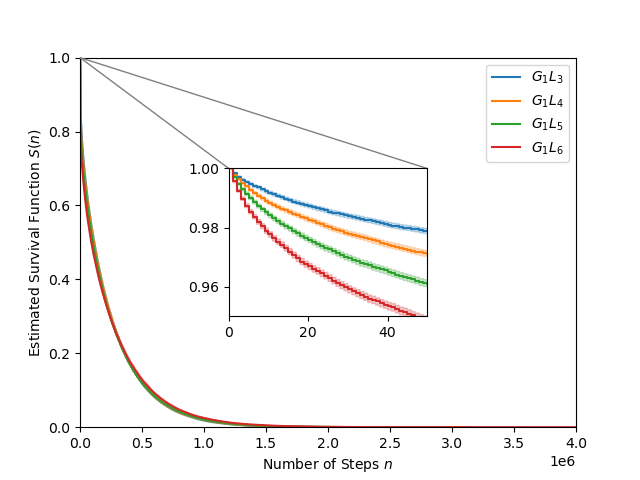
\includegraphics[width=\textwidth]{G_1_steps_sf.png}
          \caption{}
          \label{fig:sf_g1_branch_steps}
        \end{subfigure}
        \hfill
        \begin{subfigure}[b]{0.45\textwidth}
          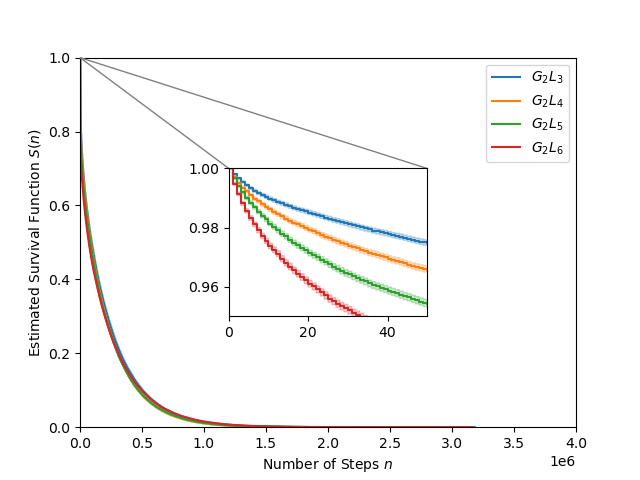
\includegraphics[width=\textwidth]{G_2_steps_sf.png}
          \caption{}
          \label{fig:sf_g2_branch_steps}
        \end{subfigure}
        \caption{(a) and (b) are survival functions for branching
          structures in $G_1$ and $G_2$, respectively. $n$ is the
          number of steps taken by the particle from the initial to
          the stop pixel in LRWs.}
        \label{fig:sf_branch_steps}
      \end{figure}

       
       The insets in Fig.~\ref{fig:sf_branch_steps} show that, within
       a group, the decay rates of $S(n)$ for $L_j$, $j=3, ..., 6$,
       are significantly distinct as $n$ approaches $0$. The graphical
       representation of short-time behaviours of survival functions
       is consistent with the analytical result since bigger $j$
       results in the larger perimeter of the branching structure.
       

       \begin{figure}
         \centering
         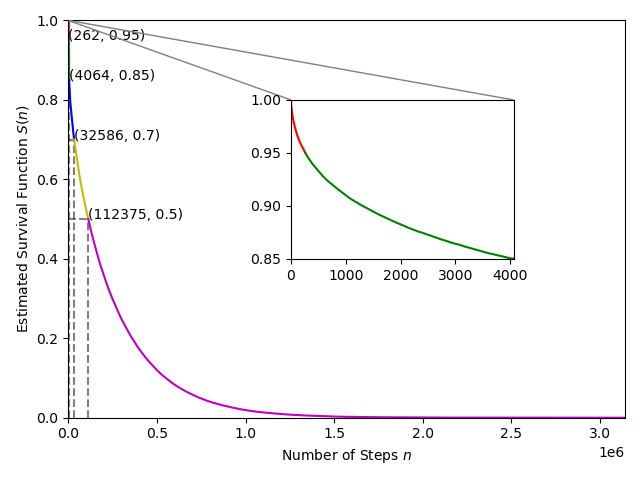
\includegraphics[width=\textwidth]{steps_seg_curve_G_1_L_3.png}
         \caption{It is an estimated survival function for LRWs in $G_1L_3$.}
         \label{fig:steps_seg_curve_G_1_L_3}
       \end{figure}

       
       As shown in Fig.~\ref{fig:steps_seg_curve_G_1_L_3}, the
       survival curve is divided into several coloured segments. In
       Fig.~\ref{fig:G_1_L_3_steps_red_initial_pos_distribution},
       Fig.~\ref{fig:G_1_L_3_steps_green_initial_pos_distribution},
       Fig.~\ref{fig:G_1_L_3_steps_blue_initial_pos_distribution},
       Fig.~\ref{fig:G_1_L_3_steps_blue_initial_pos_distribution}, and
       Fig.~\ref{fig:G_1_L_3_steps_pink_initial_pos_distribution},
       particles' initial and stop positions are painted with colour
       identical to the survival curve segment to understand the
       underlying stochastic process and its properties. Furthermore,
       the black region in the initial position plot is the target
       branching structure.

       
       
       \begin{figure}
         \centering
         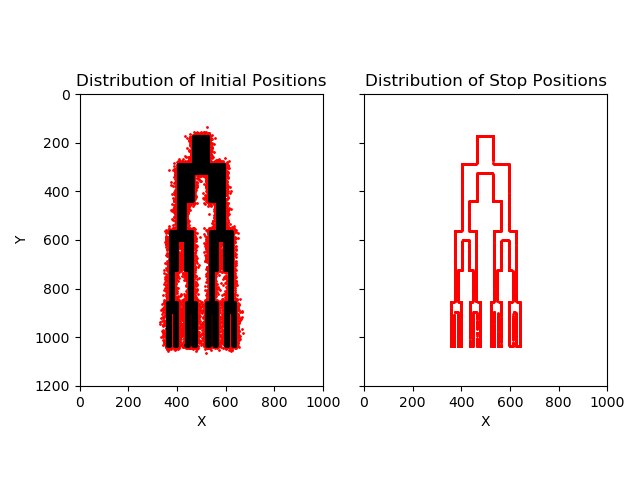
\includegraphics[width=\textwidth]{G_1_L_3_steps_red_initial_pos_distribution.png}
         \caption{$5\%$ of particles in the LRWs coloured by red will
           be absorbed within $262$ steps. In the left subfigure,
           particles' initial positions are distributed closely
           surrounding the target branching structure. The in-between
           space of tiny bottom limbs is filled with particles, while
           some area between the huge top branches is empty. The right
           subfigure shows that the red particles characterize the
           entire boundary of the object.}
         \label{fig:G_1_L_3_steps_red_initial_pos_distribution}
       \end{figure}



       \begin{figure}
         \centering
         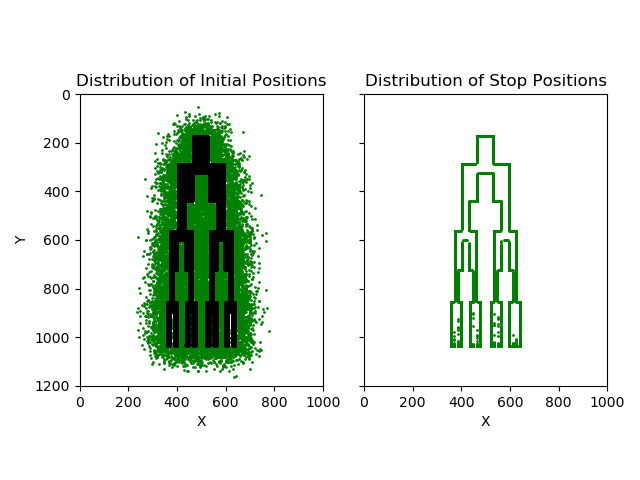
\includegraphics[width=\textwidth]{G_1_L_3_steps_green_initial_pos_distribution.png}
         \caption{Around $10$ percent of particles are generated
           adjacent to the fringe of the object, whose steps ranged
           from $262$ to $4064$. Compared with
           Fig.~\ref{fig:G_1_L_3_steps_red_initial_pos_distribution},
           the green points also dispersed thoroughly between the
           branches. Nevertheless, some in-between regions of the
           lowest branches are empty, resulting in the object's
           incompleted edge in the right plot.}
         \label{fig:G_1_L_3_steps_green_initial_pos_distribution}
       \end{figure}


       \begin{figure}
         \centering
         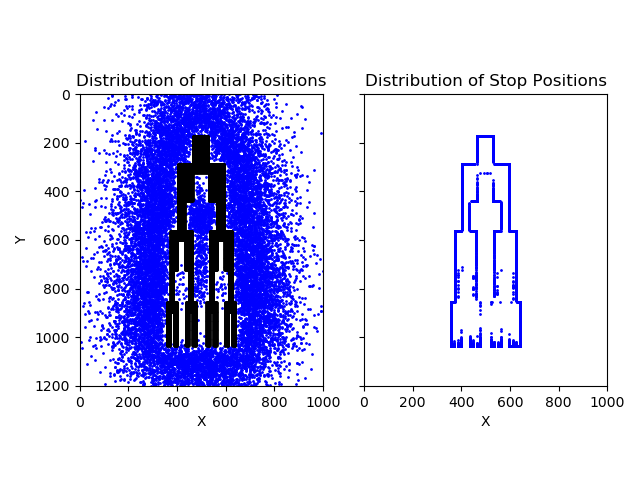
\includegraphics[width=\textwidth]{G_1_L_3_steps_blue_initial_pos_distribution.png}
         \caption{Approximate $15$ percent of particles originally
           started LRWs from the region slightly far away from the
           target object. The number of steps for the blue particles
           is from 4064 to 32586. Not like the
           Fig.~\ref{fig:G_1_L_3_steps_green_initial_pos_distribution},
           fewer blue particles are located initially between the
           narrower branches. Moreover, if particles' initial sites
           are further away from the branching structure's external
           boundary, they will be more dispersive. The particles in
           the right subfigure can depict only some top pieces of the
           internal border.}
         \label{fig:G_1_L_3_steps_blue_initial_pos_distribution}
       \end{figure}
       

       \begin{figure}
         \centering
         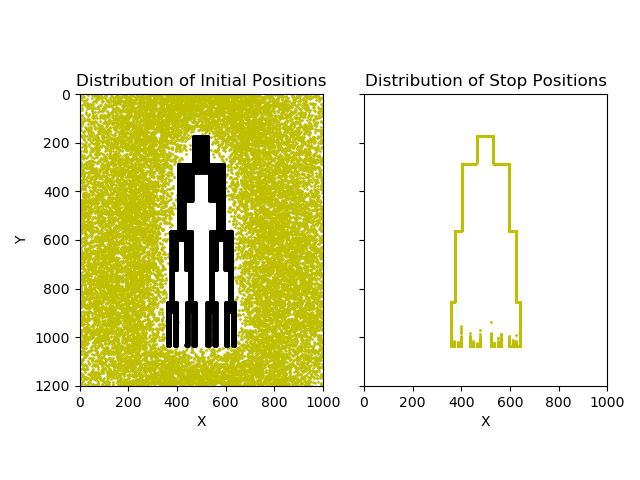
\includegraphics[width=\textwidth]{G_1_L_3_steps_y_initial_pos_distribution.png}
         \caption{The left subplot displays the initial positions of
           $60\%$ of particles in LRWs distributed uniformly in the
           empty space of the image but slightly far away from the
           target object. Moreover, none of them initially started
           LRWs from the in-between region of the branches. Compared
           with the
           Fig.~\ref{fig:G_1_L_3_steps_blue_initial_pos_distribution},
           the right subplot shows the object's entire external
           boundary and some internal boundary of its terminal limbs.}
         \label{fig:G_1_L_3_steps_yellow_initial_pos_distribution}
       \end{figure}


       \begin{figure}
         \centering
         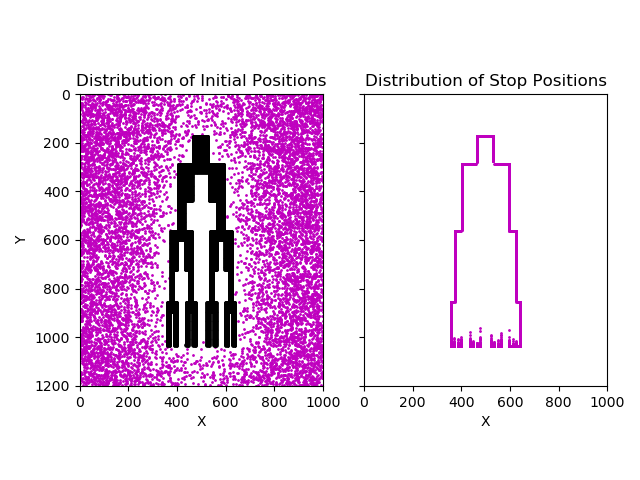
\includegraphics[width=\textwidth]{G_1_L_3_steps_m_initial_pos_distribution.png}
         \caption{Only $10$ percent of particles will survive when
           their number of steps is bigger than $549701$. They are
           distributed initially from a region far away from the
           object and close to the image's edges. Similar to
           Fig.~\ref{fig:G_1_L_3_steps_yellow_initial_pos_distribution},
           pink particles cannot delineate too much internal boundary
           of the branching structure.}
         \label{fig:G_1_L_3_steps_pink_initial_pos_distribution}
       \end{figure}



       In reality, LRWs is latent and cannot be observed
       directly. However, those scatter plots are helpful to reveal
       the first-passage properties of particles in LRWs. For
       instance, particles will be absorbed within a smaller number of
       steps if their starting positions are closer to the target
       because they have less randomness. Moreover, more particles
       will be generated in the broader and longer in-between area of
       branches. Therefore, each segment of the survival curve carries
       massive geometric and spatial information about the unoccupied
       area of the binary image (i.e. the region with black pixels)
       and the boundary of the simply connected domain (i.e. the
       artificial branching structure with white pixels).



       \begin{figure}
        \centering
        \begin{subfigure}[b]{0.45\textwidth}
          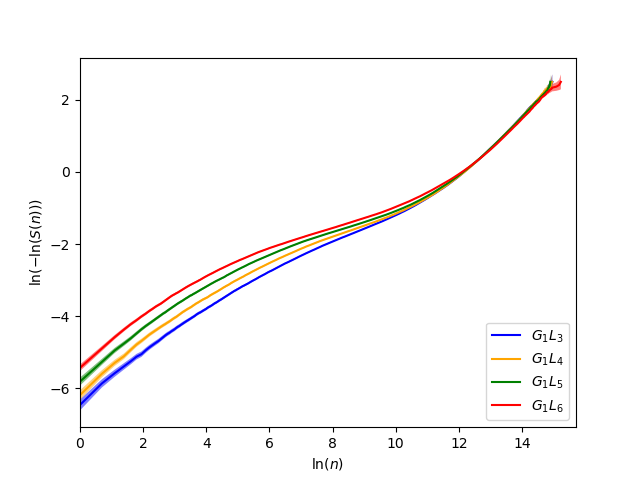
\includegraphics[width=\textwidth]{G_1_steps_check_ph.png}
          \caption{}
          \label{fig:g1_steps_check_ph}
        \end{subfigure}
        \hfill
        \begin{subfigure}[b]{0.45\textwidth}
          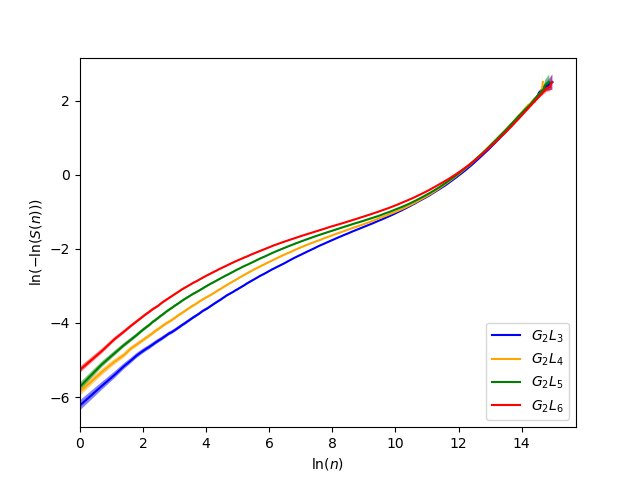
\includegraphics[width=\textwidth]{G_2_steps_check_ph.png}
          \caption{}
          \label{fig:g1_steps_check_ph}
        \end{subfigure}
        \caption{(a) and (b) are commonly used graphical techniques to
          check the proportional hazards (PH) assumption of survival data
          by finding the parallelism. The survival distributions do
          not support the PH assumption since the
          hazard ratio in both $G_1$ and $G_2$ is not always constant.}
        \label{fig:branch_steps_check_ph}
       \end{figure}
       
             
      \begin{table}
        \centering
        \begin{tabular}{llrrrr}
          \toprule
                       &             &         &  p &    &     \\
          \cmidrule{3-6}
                       &             & Log-rank & TW & GB & FH  \\
          \midrule
          $G_1$ $L_3$  & $G_1$ $L_4$  &  0.4393 &  0.0285 &  0.0005 &  0.0005     \\
                       & $G_1$ $L_5$  & 0.0 & 0.0 & 0.0 & 0.0    \\
                       & $G_1$ $L_6$  & 0.0 & 0.0 & 0.0 & 0.0      \\
          $G_1$ $L_4$  & $G_1$ $L_5$  & 0.0007 & 0.0 & 0.0 & 0.0      \\
                       & $G_1$ $L_6$  & 0.0002 & 0.0 & 0.0 & 0.0       \\
          $G_1$ $L_5$   & $G_1$ $L_6$ & 0.7223 &  0.0 & 0.0 & 0.0      \\
          \bottomrule
        \end{tabular}
        \caption{The differences between the pairwise survival
          functions for branching objects in $G_1$ are statistically
          significant based on TW, GB, and FH tests.}
         \label{tab:g1_ingroup_tests_steps}
      \end{table}


      \begin{table}
        \centering
        \begin{tabular}{llrrrr}
          \toprule
                       &             &         &  p &    &     \\
          \cmidrule{3-6}
                       &             & Log-rank & TW & GB & FH  \\
          \midrule
          $G_2$ $L_3$  & $G_2$ $L_4$  &  0.0 &  0.0 &  0.0 &  0.0     \\
                       & $G_2$ $L_5$  & 0.0 & 0.0 & 0.0 & 0.0    \\
                       & $G_2$ $L_6$  & 0.0 & 0.0 & 0.0 & 0.0      \\
          $G_2$ $L_4$  & $G_2$ $L_5$  & 0.0016 & 0.0 & 0.0 & 0.0      \\
                       & $G_2$ $L_6$  & 0.0004 & 0.0 & 0.0 & 0.0       \\
          $G_2$ $L_5$   & $G_2$ $L_6$ & 0.7199 &  0.0 & 0.0 & 0.0      \\
          \bottomrule
        \end{tabular}
        \caption{It is well known that the log-rank test will lose
          power if the proportional hazard assumption is
          violated. Except for the log-rank test, other statistical
          tests indicate that the pairwise survival functions for
          branching objects in $G_2$ are statistically different.}
        \label{tab:g2_ingroup_tests_steps}
      \end{table}
      

      Some weighted log-rank tests can be utilized to detect the early
      or late differences between the pairwise overlapping or crossing
      survival curves. In Table ~\ref{tab:g1_ingroup_tests_steps} and
      Table ~\ref{tab:g2_ingroup_tests_steps}, TW is the abbreviation
      for Tarone-Ware test, GB is for Gehan-Breslow test, and FH is
      for Fleming-Harrington test. However, p values in the tables are
      not too informative, and the log-rank test under conditions of
      non-proportional hazards leads to misleading results. Hence,
      distance measures are alternative methodologies for quantifying
      the discrepancy between survival functions.
      

      It is assumed that $\widehat S_1(t)$ and $\widehat S_2(t)$ are
      the Kaplan-Meier estimators of the survival functions for random
      variable $T_1 > 0$ and $T_2 > 0$, respectively. Let
      $(\tau_j)_{j=1, 2, ..., N}$ are distinct increasing observed
      times when the event of interest take place. In the vector
      space, the distance between $\widehat S_1(t)$ and $\widehat
      S_2(t)$ can be defined as the $L_p$ norm of their difference, $
      1 \leq p \leq \infty$, where

      \begin{equation}\label{eq:lp_norm}
        \begin{split}
          d_p(\widehat S_1(t), \widehat S_2(t))&= \lVert \widehat S_1(t) - \widehat S_2(t) \rVert_{p} \\
          &= \Big(\sum^{N}_{j=1} \lvert \widehat S_1(\tau_j) - \widehat S_2(\tau_j)\rvert^p\Big)^{\frac{1}{p}} \\
          &= \Big(\sum^{N}_{j=1} \lvert P({T_1 > \tau_j}) - P({T_2 > \tau_j}) \rvert^p\Big)^{\frac{1}{p}}
        \end{split}
      \end{equation}
      
      
      \begin{figure}
        \centering
        \begin{subfigure}[b]{0.45\textwidth}
          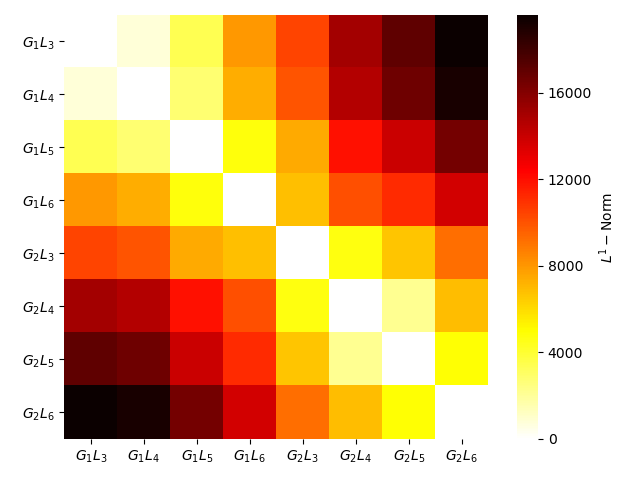
\includegraphics[width=\textwidth]{heatmap_ai_steps_l1.png}
          \caption{}
          \label{fig:heatmap_ai_steps_l1}
        \end{subfigure}
        \begin{subfigure}[b]{0.45\textwidth}
          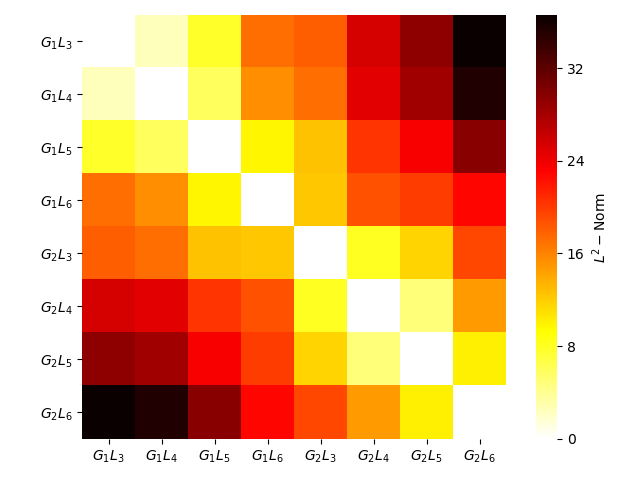
\includegraphics[width=\textwidth]{heatmap_ai_steps_l2.png}
          \caption{}
          \label{fig:heatmap_ai_steps_l2}
        \end{subfigure}
        \caption{The distance matrices of pairwise survival functions for artificial images are visualized by heat maps.}
        \label{fig:heatmap_ai_steps}
      \end{figure}


      Let $p$ be $1$ and $2$ in Eq.~\ref{eq:lp_norm} respectively, the
      distance between a pair of survival functions is measured by
      $d_1$ and $d_2$, and is depicted by colors in the heat maps as
      shown in Fig.~\ref{fig:heatmap_ai_steps_l1} and
      Fig.~\ref{fig:heatmap_ai_steps_l2}. The cells on the main
      diagonal are white because the distance of an object from itself
      is zero. Moreover, the off-diagonal cells are symmetric. The
      darker cells in the heat maps demonstrate more significant
      dissimilarities between survival functions or curves. In other
      words, the colour of cells describes the variation in the shapes
      of branching structures in artificial images.


      The top left and bottom right $4 \times 4$ cells are the
      in-group shape comparison of the branching structures. For each
      column, the cells become darker gradually since the objects in
      each group are more complicated as $j$ increase. The pale yellow
      cells adjacent to the diagonal, including $(G_1L_3, G_1L_4)$,
      $(G_1L_4, G_1L_5)$, $(G_1L_5, G_1L_6)$, $(G_2L_3, G_2L_4)$,
      $(G_2L_4, G_2L_5)$, and $(G_2L_5, G_2L_6)$, imply that the
      morphological changes are not dramatically different. Moreover,
      the top right and bottom left $4 \times 4$ cells are the
      between-group shape comparison. The smaller dissimilarities are
      closer to the diagonal, which gives a form of clustering the
      artificial images.

      
      Metric Multidimensional scaling (MDS) \cite{borg2005modern} is
      employed to display the distance matrix using a map defined in
      an abstract Cartesian space. Given a dimension $p$ and a
      distance matrix $D = (d_{ij})$, MDS is used to find a
      configuration $\bm{x_1}, ..., \bm{x_n} \in \mathbb{R}^p$, which
      satisfies

      \begin{equation}\label{eq:mMDS}
        f(d_{ij}) \approx \widehat{d}_{ij} = \lVert \bm{x_i} - \bm{x_j} \lVert_{2}
      \end{equation}

      as close as possible, and $f$ could be a parametric monotonic function, such as $f(d_{ij}) = \alpha + \beta d_{ij}$.

      Metric MDS aims to minimizes the stress denoted by $\mathcal{L}(\widehat{d}_{ij})$ over all $\widehat{d}_{ij}$, $\alpha$, and $\beta$,

      \begin{equation}\label{eq:stress_mMDS}
        stress = \mathcal{L}(\widehat{d}_{ij}) = \bigg( \sum_{i<j} (\widehat{d}_{ij} - f(d_{ij}))^2 / \sum d^2_{ij} \bigg)^{\frac{1}{2}}
      \end{equation}
      

      In Fig.~\ref{fig:MDS_ai_steps_l1} and
      Fig.~\ref{fig:MDS_ai_steps_l2}, MDS denotes the artificial
      images as points in $2-$ dimensional geometric space so that
      distances between pairs of points match as well as possible the
      original dissimilarities calculated between the pairwise
      survival functions. Moreover, the axes in themselves are
      meaningless. For metric scaling \cite{scikit-learn}, a smaller
      stress $\mathcal{L}(\widehat{d}_{ij})$ indicates a better fit of
      the configuration. Generally, a value of the stress of $20\%$
      suggests a poor fit, $10\%$ fair, $5\%$ good and $2\%$ an
      excellent fit.
       

      \begin{figure}
        \centering
        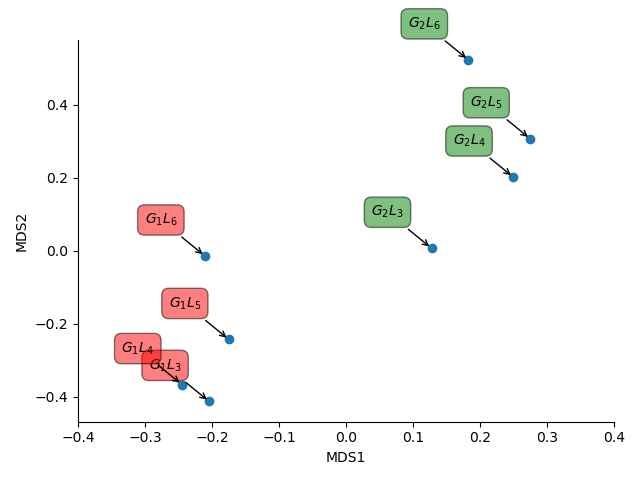
\includegraphics[width=\textwidth]{MDS_ai_steps_l1.png}
        \caption{It is the MDS of the distance matrix calculated based
          on $d_1$, and the stress for the plot is about $0.82\%$. Points
          with green labels in the bottom left-hand corner illustrate
          the $G_1$ images, while others are $G_2$ images. It is easy
          to tell that there are two clusters for the artificial
          images, which coincide with reality and heat map in
          Fig.~\ref{fig:heatmap_ai_steps_l1}.}
        \label{fig:MDS_ai_steps_l1}
      \end{figure}



      \begin{figure}
        \centering
        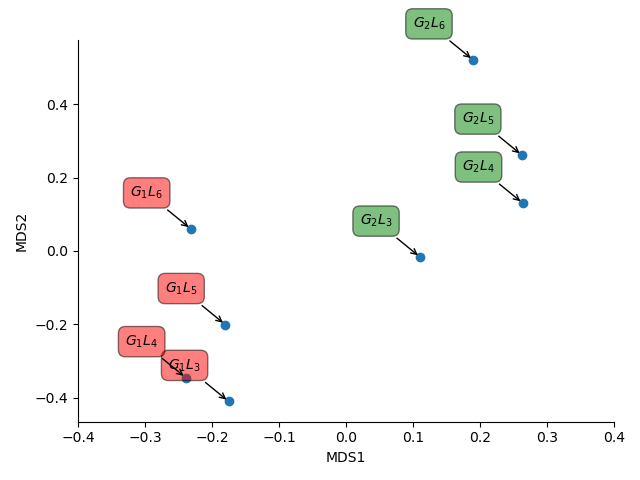
\includegraphics[width=\textwidth]{MDS_ai_steps_l2.png}
        \caption{It is the MDS plot of the distance matrix calculated
          by $d_2$ with the stress $0.4\%$.}
        \label{fig:MDS_ai_steps_l2}
      \end{figure}

      
      



       



       


























      
